\subsubsection{Sveska 11}

\zadatak
Re{\sv}i nejedna{\cv}inu
$$
\log_3^2 x - 5\log_3  x + 6 \le 0.
$$

\resenje
Kada izvr{\sv}imo smenu $t=\log_3 x$, mo{\zv}emo pisati da je
$$
t^2-5t+6\le0
$$
Kako su re{\sv}e{\nj}a kvadratne jedna{\cv}ine\queq\ $t_1=2$ i $t_2=3$,
nejedna{\cv}ina je zadovo{\lj}ena kada je $t\in[2,3]$. \
Po{\sv}to je $x=3^t$, sledi da je nejedna{\cv}ina zadovo{\lj}ena za
$x\in[3^2,3^3]$, odnosno,
$$
\ram{9\le x\le 27}.
$$
\vskip-36pt
$$
\slika{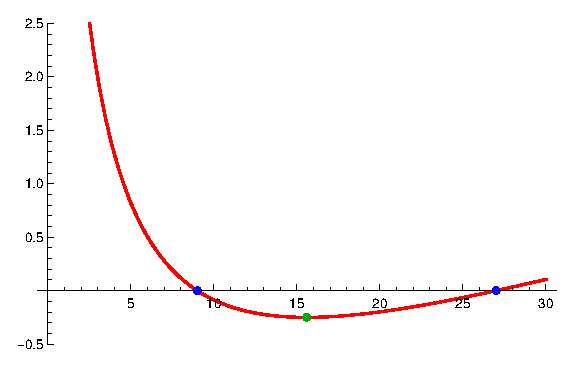
\includegraphics[width=\sirina]{eps/11.eps}}{$y=\log_3^2 x - 5\log_3  x + 6$.}
$$

\dodatak Funkcija ima \idx{minimum} za $t=5/2$, odnosno, u ta{\cv}ki $(9\sqrt3,-1/4)$.